\section{Network}\label{sec:network}

Our network architecture contains two copies of odd-one-out network in order to learn both temporal order and smoothness at the same time. 
The input frames are sampled from sequenced videos with $N+1$ input clips for each odd-one-out network.
As mentioned in the previous section, only one out of the $N+1$ clips is out of order. 
Furthermore, two clips that are chronological close in the same video are used to feed the two copies of odd-one-out network. 
Figure~\ref{fig:network} is a demonstration with $N=1$.
In particular, clips from the same sequence of video, such as $c_0$ and $c_0\rq{}$, are inputs for the two odd-one-out networks seperately.  
For each odd-one-out network, only one clip is out of order, such as either $c_0$ or $c_1$ for the \lq\lq{}left\rq\rq{} network.

This network architecture makes it possible to consider out-of-order loss $L_{O3N}$ and temporal smoothness loss $L_T$ at the same time. 
Both losses have been discussed in previous sections, and can be conbined as loss for the proposed network:
$$L = L_{O3N} + \gamma L_T$$
where hyperparameter $\gamma$ captures the priority between the two losses. 
This paper is the first attempt to combine odd-one-out learning with temporal cohence, and a non-trivial choice of $\gamma$ provides insights to the effectiveness of this learning strategy.

\begin{figure}
\centering
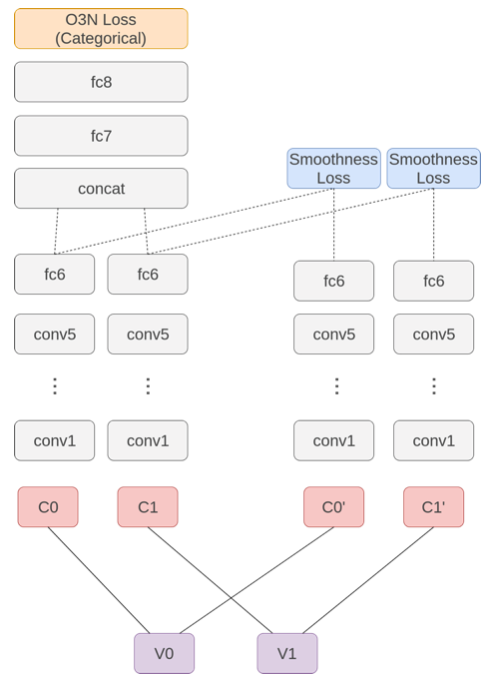
\includegraphics[width=0.35\textwidth]{images/network.png}
\caption{Network architecture.}
\label{fig:network}
\end{figure}